\section{General Description}
\paragraph{Xilinx Zynq UltraScale+ RFSoC ZCU216 Evaluation Card}
Zynq UltraScale+ RFSoCs: Combine RF data converter subsystem and forward error correction with industry-leading
programmable logic and heterogeneous processing capability. Integrated RF-ADCs, RF-DACs, and soft decision FECs (SD-FEC)
provide the key subsystems for multiband, multi-mode cellular radios and cable infrastructure


The card, holding the sampling channels, should be mounted on a ZCU216 evaluation board. This board is the newest generation of Xilinx' evaluation cards, which has features suitable for the purpose at hand.
\begin{itemize}[noitemsep]
	\item Sixteen 14-bit, 2.5GSPS RF-ADC
	\item Sixteen 14-bit, 10GSPS RF-DAC
	\item I/O expansion options – FPGA Mezzanine Card (FMC+) interfaces, RFMC 2.0 interfaces, and Pmod connections
\end{itemize}
\begin{figure}[tbh]
	\centering
	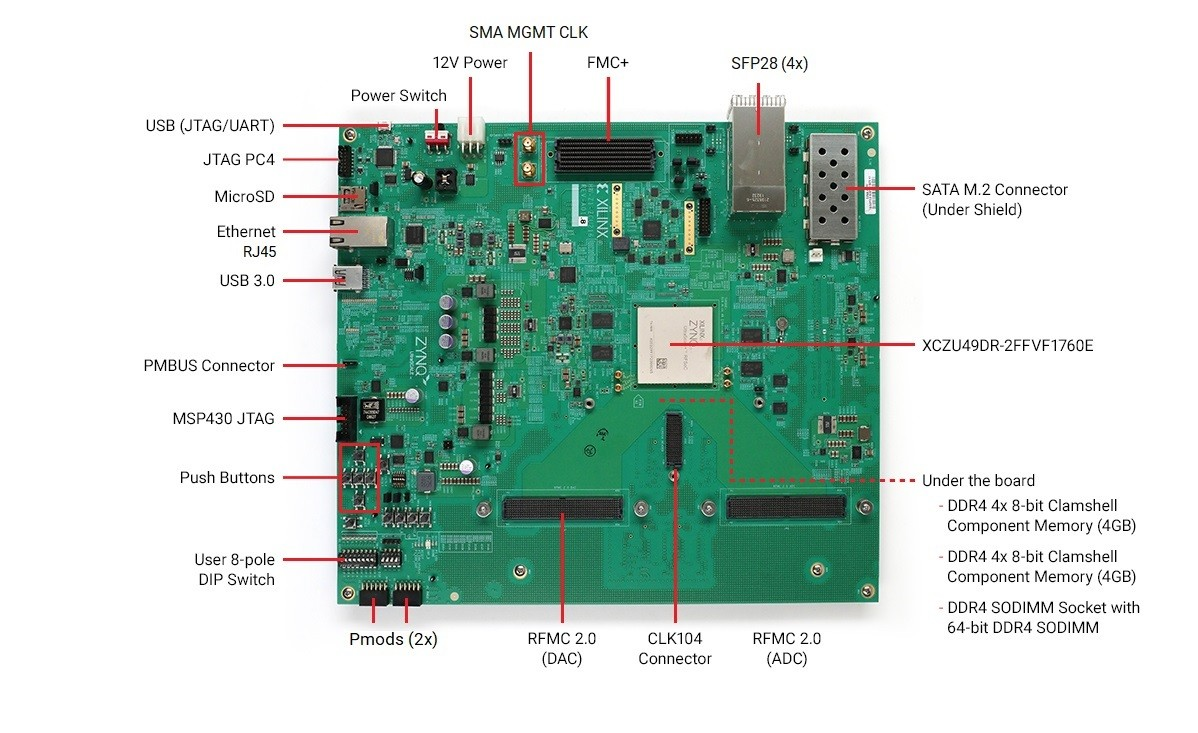
\includegraphics[width = \textwidth]{chap/04-work/img/zcu216}
	\caption{ZCU216 evaluation board}
	\label{fig:zcu216}
\end{figure}

\begin{figure}[tbh]
	\centering
	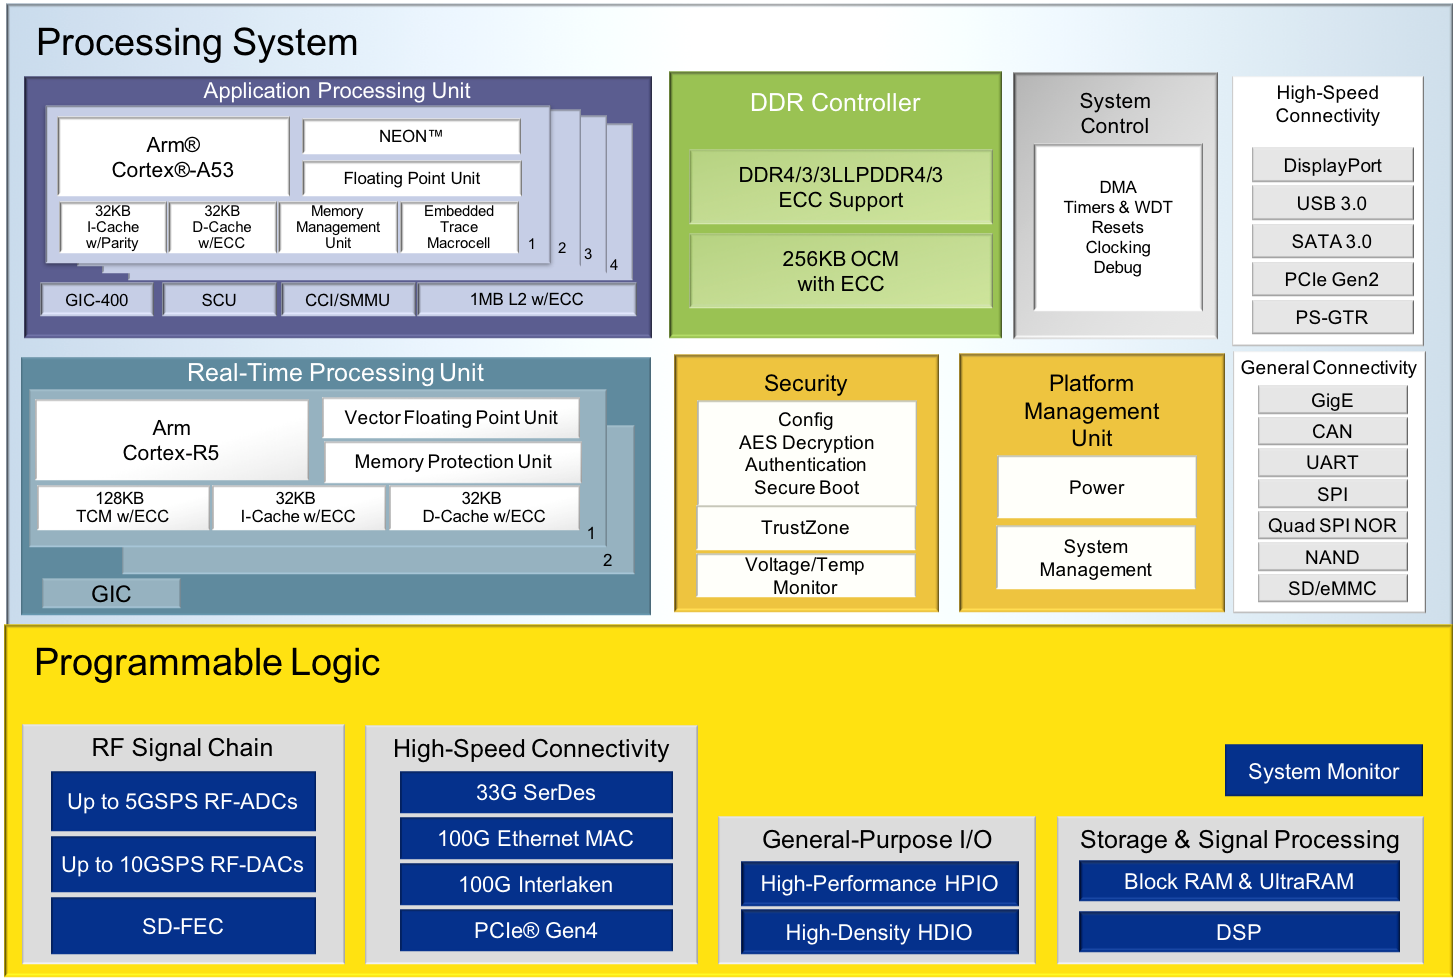
\includegraphics[width = \textwidth]{chap/04-work/img/rfsoc_blockdiagram}
	\caption{RFSoC block diagram}
	\label{fig:rfsoc}
\end{figure}
\section{Features}